\begin{exercício}{Molécula triatômica linear}{exercício1}
    Considere os estados de um elétron de uma molécula triatômica linear formada de átomos \(E, C, \) e \(D\); as distâncias \(EC\) e \(CD\) o iguais e de valor \(d\).
    \begin{center}
        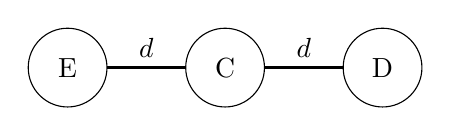
\begin{tikzpicture}
            \def\d{2}
            \draw (0, 0) circle(0.5) node at (0, 0) {E};
            \draw (\d, 0) circle(0.5) node at (\d, 0) {C};
            \draw (2*\d, 0) circle(0.5) node at (2*\d, 0) {D};
            \draw[thick] (0.5, 0) -- (\d-0.5, 0) node[midway, above]{\(d\)};
            \draw[thick] (\d+0.5, 0) -- (2*\d-0.5, 0) node[midway, above]{\(d\)};
        \end{tikzpicture}
    \end{center}
    Designamos por \(\ket{\psi_E}, \ket{\psi_C}\) e \(\ket{\psi_D}\) os autovetores normalizados do operador \(B\), correspondentes ao elétron localizado respectivamente na vizinhança dos átomos \(E, C,\) e \(D\)
    \begin{align*}
        B\ket{\psi_E} &= - d\ket{\psi_E}&
        B\ket{\psi_C} &= 0&
        B\ket{\psi_D} &= d\ket{\psi_D}.
    \end{align*}
    Quando ignoramos a possibilidade do elétron saltar de um átomo para outro, sua energia é designada pelo hamiltoniano \(H_0\) que admite como autovetores os estados \(\ket{\psi_E}, \ket{\psi_C}, \ket{\psi_D}\) com o mesmo autovalor \(E_0\). O acoplamento entre os estados \(\ket{\psi_E}, \ket{\psi_C}, \ket{\psi_D}\) é descrito por um hamiltoniano suplementar \(W\) definido por
    \begin{align*}
        W \ket{\psi_E} &= -a \ket{\psi_C}&
        W \ket{\psi_C} &= -a \ket{\psi_E} - a \ket{\psi_D}&
        W \ket{\psi_D} &= -a \ket{\psi_C},
    \end{align*}
    onde \(a > 0\).
    \begin{enumerate}[label=(\alph*)]
        \item Calcule os níveis de energia e os autoestados de \(H = H_0 + W\).
        \item Considere o estado fundamental; quais as probabilidades de encontrar o elétron em \(E, C\) e \(D\)?
        \item Considere um elétron no estado \(\ket{\psi_E}\). Se medirmos sua energia, que valores podemos encontrar? Quais as probabilidades de cada valor?
        \item Calcule o valor médio e o desvio padrão da energia para o estado \(\ket{\psi_E}.\)
    \end{enumerate}
\end{exercício}
\begin{proof}[Resolução ]

\end{proof}
